\documentclass[aps,superscriptaddress,groupedaddress]{revtex4}  % for double-spaced preprint

\usepackage{graphicx}  % needed for figures
\usepackage{float}
\usepackage{dcolumn}   % needed for some tables
\usepackage{bm}        % for math
\usepackage{amssymb}   % for math
\usepackage{slashed}   % for Dirac Slash
\usepackage{amsmath}   % for mutiline eqn
\usepackage{simplewick} % for contraction
\usepackage{verbatim}  % for multi-line comment
\usepackage{color} % for textcolor
\usepackage{appendix} % for appendix
\usepackage{epstopdf}
\usepackage{subfig}
\usepackage{listings}
\usepackage{xcolor}

% \usepackage[numbers,sort&compress]{natbib} %for cite

% avoids incorrect hyphenation, added Nov/08 by SSR
\hyphenation{ALPGEN}
\hyphenation{EVTGEN}
\hyphenation{PYTHIA}

% for bookmarks
\usepackage[bookmarks=true,colorlinks=true,linkcolor=blue,unicode=true]{hyperref}

\begin{document}

\widetext

\title{Manual of pre-built}

\date{\today}


\begin{abstract}
Manual of pre-built
\end{abstract}

\maketitle

\section{\label{sec:1}Run simulation}

The number of the lattice are $512\times 512$.

Before run simulation, one have to set the exchange strength, magnetic momentum and boundary condition, using the button shown in Fig.~\ref{Fig:intro1}.
\begin{figure}
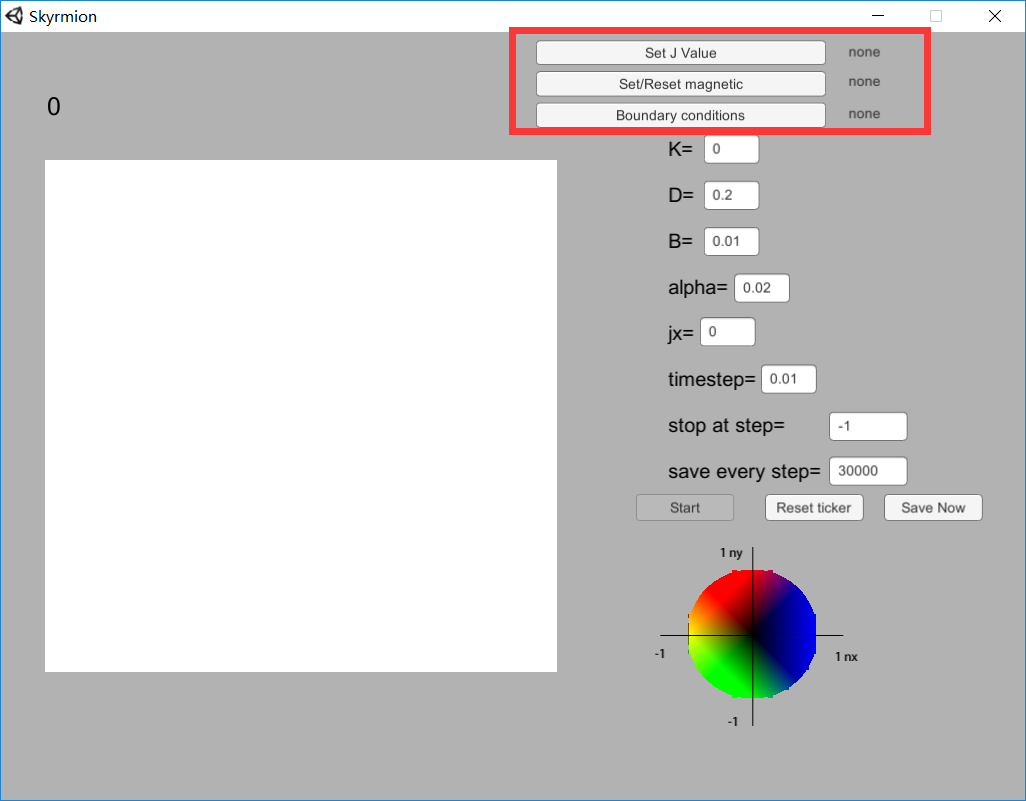
\includegraphics[scale=0.3]{intro1.png}
\caption{\label{Fig:intro1}Set the exchange strength, magnetic momentum and boundary condition.}
\end{figure}

The exchange strength is a lua script generate $J$ for every lattice index. It is introduced in Sec.~\ref{sec:2}.

The magnetic momentum can be either a lua script or a image file introduced in Sec.~\ref{sec:3}.

The boundary condition is a image file introduced in Sec.~\ref{sec:4}.

Then set the parameters as shown in Fig.~\ref{Fig:intro2}.
\begin{figure}
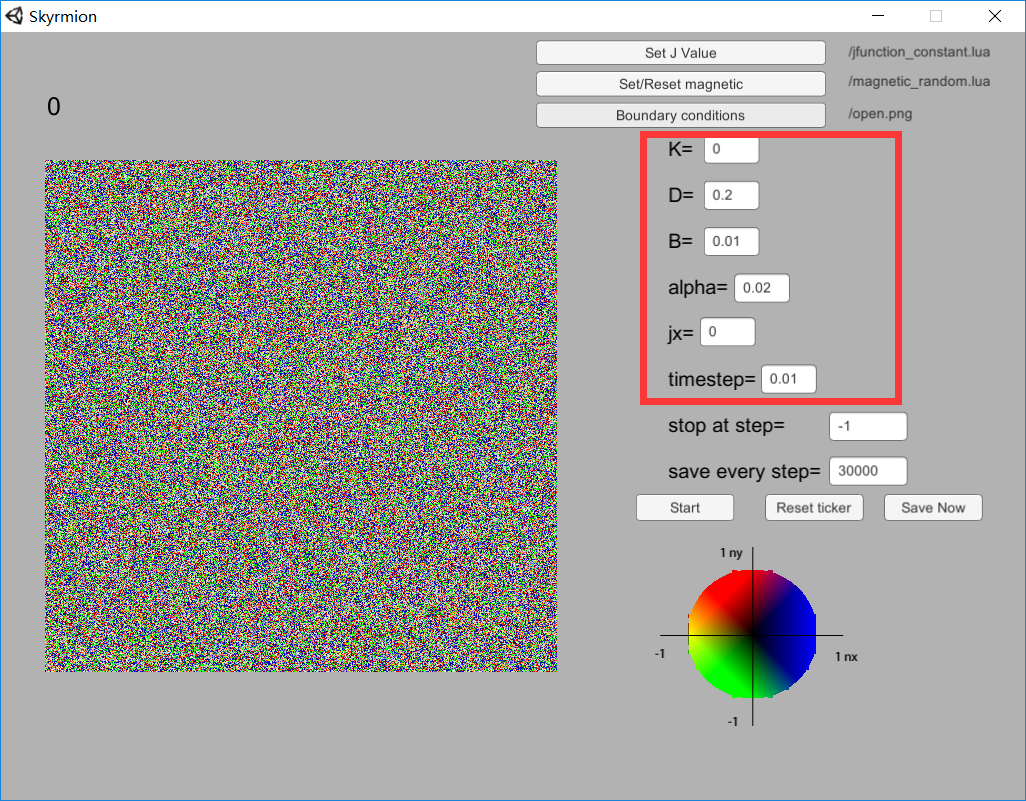
\includegraphics[scale=0.3]{intro2.png}
\caption{\label{Fig:intro2}Set other parameters.}
\end{figure}

The simulation can be paused at any time, when paused, all the parameters can be changed. The simulation can also been stopped automatically. It is shown in Fig.~\ref{Fig:intro3}. When $step = stop\;at\;step$, it will stop, and when $step \mod save\;every\;step=0$, the data is saved automatically. Using the configure in Fig.~\ref{Fig:intro3}, the simulation will not stop automatically, and the state of the magnetic momentum will be saved when steps are $0,30000,60000,\ldots$. The output files are introduced in Sec.~\ref{sec:5}.
\begin{figure}
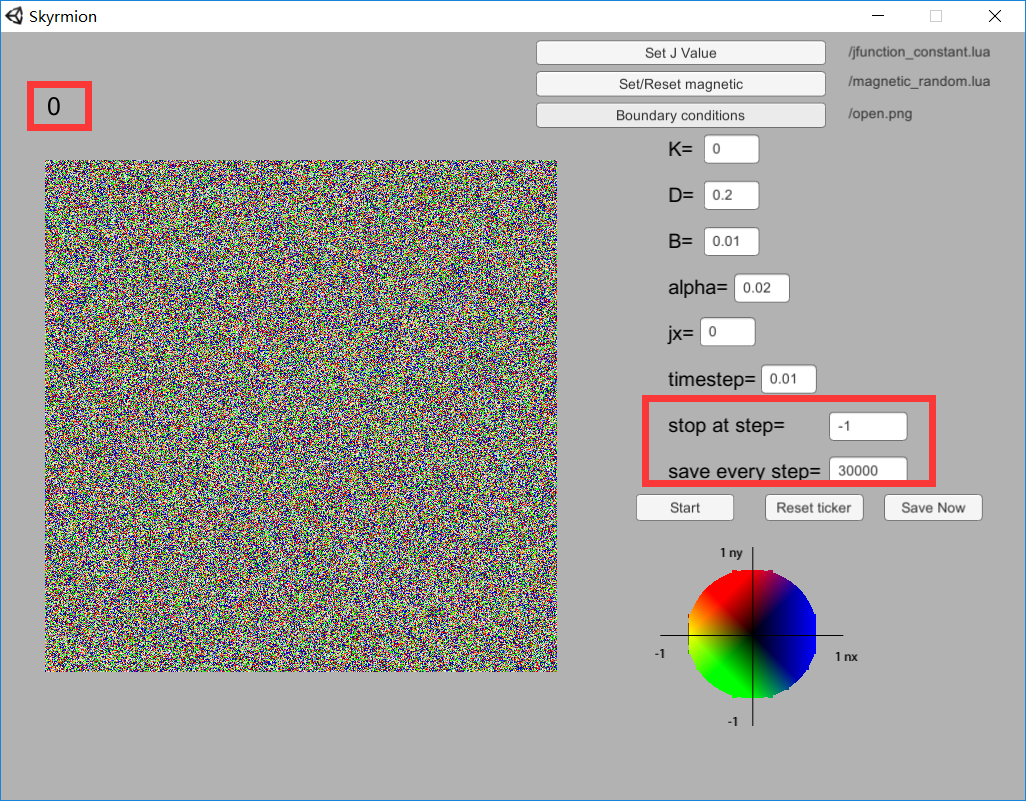
\includegraphics[scale=0.3]{intro3.png}
\caption{\label{Fig:intro3}Set stop steps. The number in left-up corner is the number of step.}
\end{figure}

The configuration of above will generate results shown in Fig.~\ref{fig:result}.
\begin{figure}[htb]
\centering
\subfloat[$step=0$]{
\includegraphics[width=0.16\textwidth]{4-3-15-14_0_show.png}}\hfill
\subfloat[$step=300000$]{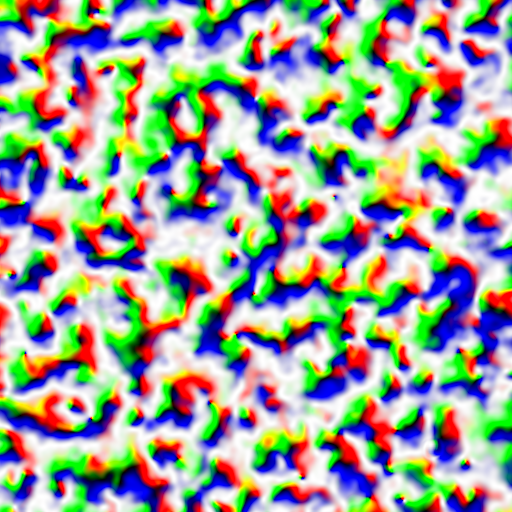
\includegraphics[width=0.16\textwidth]{4-3-15-14_300000_show.png}}\hfill
\subfloat[$step=600000$]{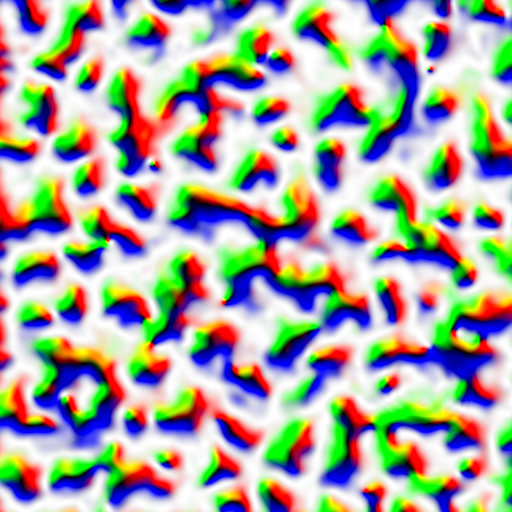
\includegraphics[width=0.16\textwidth]{4-3-15-14_600000_show.png}}\hfill
\subfloat[$step=900000$]{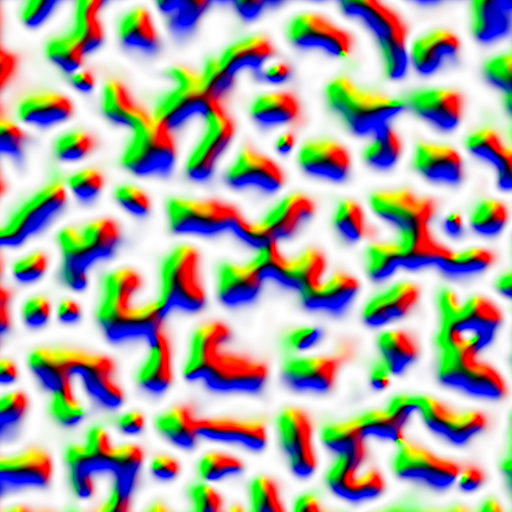
\includegraphics[width=0.16\textwidth]{4-3-15-14_900000_show.png}}\hfill
\subfloat[$step=1200000$]{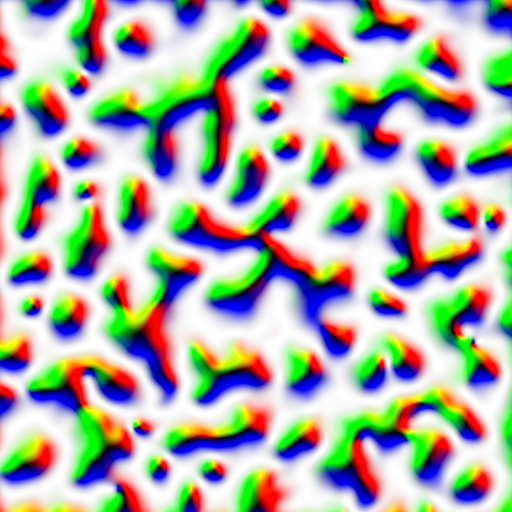
\includegraphics[width=0.16\textwidth]{4-3-15-14_1200000_show.png}}\hfill
\subfloat[$step=1500000$]{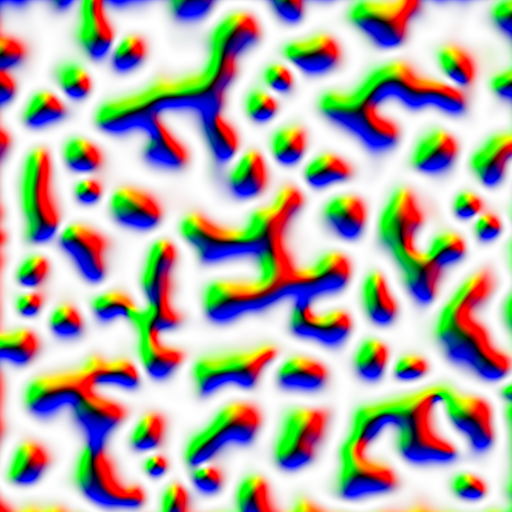
\includegraphics[width=0.16\textwidth]{4-3-15-14_1500000_show.png}}\vfill
\subfloat[$step=1800000$]{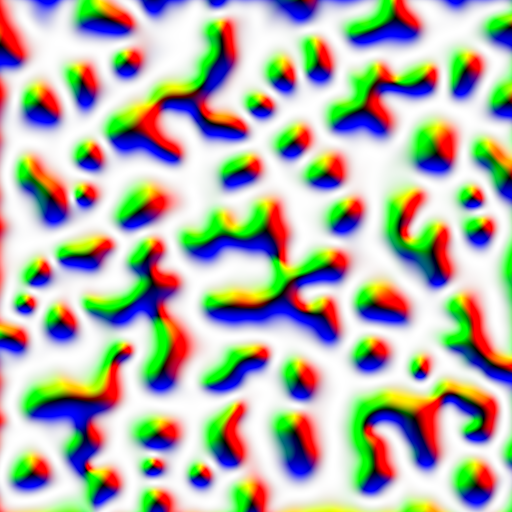
\includegraphics[width=0.16\textwidth]{4-3-15-14_1800000_show.png}}\hfill
\subfloat[$step=2100000$]{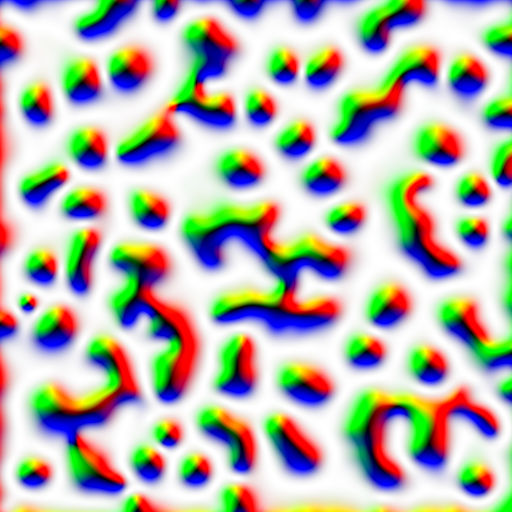
\includegraphics[width=0.16\textwidth]{4-3-15-14_2100000_show.png}}\hfill
\subfloat[$step=2400000$]{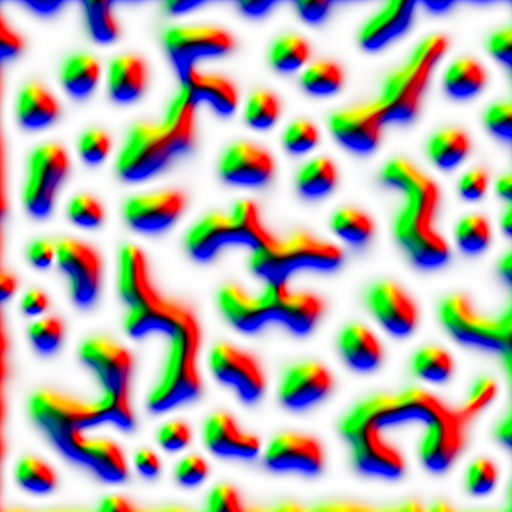
\includegraphics[width=0.16\textwidth]{4-3-15-14_2400000_show.png}}\hfill
\subfloat[$step=2700000$]{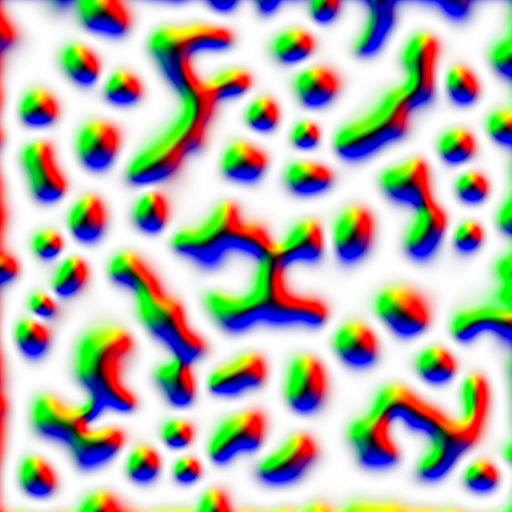
\includegraphics[width=0.16\textwidth]{4-3-15-14_2700000_show.png}}\hfill
\subfloat[$step=3000000$]{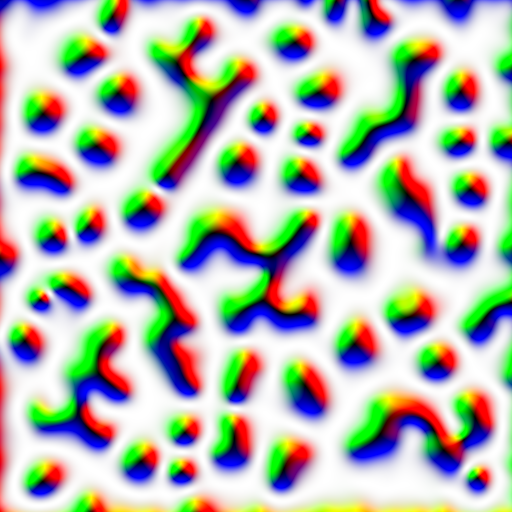
\includegraphics[width=0.16\textwidth]{4-3-15-14_3000000_show.png}}\hfill
\subfloat[$step=3300000$]{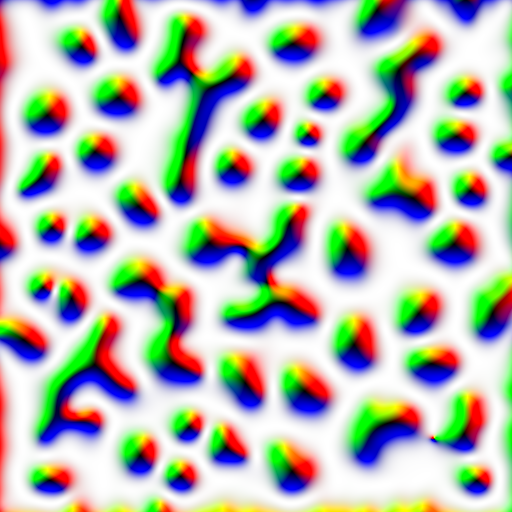
\includegraphics[width=0.16\textwidth]{4-3-15-14_3300000_show.png}}
\caption{Results}
\label{fig:result}
\end{figure}


\section{\label{sec:2}Exchange strength}

The exchange strength is a lua script with a function `GetJValueByLatticeIndex', and return a table with the function. For example, a constant exchange strength $J=2$ can be written as
\lstset{
    numbers=left,
    numberstyle= \tiny,
    keywordstyle= \color{ blue!70},
    commentstyle= \color{red!50!green!50!blue!50},
    frame=single,
    rulesepcolor= \color{ red!20!green!20!blue!20} ,
    escapeinside=``,
    xleftmargin=2em,xrightmargin=2em, aboveskip=1em,
    framexleftmargin=2em,
    language=[5.3]Lua,
    breaklines=true,
    columns=fullflexible,
    captionpos=b,
    basicstyle=\footnotesize\ttfamily,
}

\begin{lstlisting}
-- Exchange Strength is constant
function GetJValueByLatticeIndex(x, y)
    return 2.0
end

-- Need to register the function
return {
    GetJValueByLatticeIndex = GetJValueByLatticeIndex,
}
\end{lstlisting}
while a pin with $J=1+\exp \left(-0.001 \rho ^2\right)$ at lattice index $(255, 255)$ can be written as
\begin{lstlisting}
-- Exchange Strength is pin
function GetJValueByLatticeIndex(x, y)
    local j0 = 1
    local j1 = 1
    local j2 = 0.001
    local rho = (x - 255) * (x - 255) + (y - 255) * (y - 255)

    return j0 + j1 * math.exp(-1.0 * j2 * rho)
end

-- Need to register the function
return {
    GetJValueByLatticeIndex = GetJValueByLatticeIndex,
}
\end{lstlisting}

The lua files are put in 'LuaScript` sub-folder in the folder of the executable file.

\section{\label{sec:3}Magnetic momentum}

The magnetic momentums can be initialized or reset using a lua script, with a function 'GetMagneticByLatticeIndex`, and return the table with the function.

For example, random magnetic momentums can be written as
\begin{lstlisting}
-- Initial the magnetic by random
function GetMagneticByLatticeIndex(x, y)
    local nx = math.random() * 2.0 - 1.0
    local ny = math.random() * 2.0 - 1.0
    local nz = math.random() * 2.0 - 1.0
    local length_inv = 1.0 / math.sqrt(nx * nx + ny * ny + nz * nz)
    length_inv = math.max(length_inv, 0.000000001)
    return nx * length_inv, ny * length_inv, nz * length_inv
end

-- Need to register the function
return {
    GetMagneticByLatticeIndex = GetMagneticByLatticeIndex,
}
\end{lstlisting}
The magnetic momentums pointing up can be written as
\begin{lstlisting}
-- Initial the magnetic by point up
function GetMagneticByLatticeIndex(x, y)
    return 0, 0, 1
end

-- Need to register the function
return {
    GetMagneticByLatticeIndex = GetMagneticByLatticeIndex,
}

\end{lstlisting}
The magnetic momentums of a skyrmion at $100,255$ can be written as
\begin{lstlisting}
-- Initial the magnetic by random
function GetMagneticByLatticeIndex(x, y)
    -- skyrmion at position 100, 255
    local rho = (x - 100) * (x - 100) + (y - 255) * (y- 255)
    -- radius 20
    local theta = math.pi * math.exp(- rho / (20 * 20))
    local phi = math.atan2(x - 100, y - 255)

    local nx = math.cos(phi) * math.sin(theta)
    local ny = math.sin(phi) * math.sin(theta)
    local nz = math.cos(theta)

    return nx, ny, nz
end

-- Need to register the function
return {
    GetMagneticByLatticeIndex = GetMagneticByLatticeIndex,
}
\end{lstlisting}

The magnetic momentum can also been initialized or reset using a $512\times 512$ image, with color $R=n_x\times 0.5+0.5$, $G=n_x\times 0.5+0.5$, $B=n_x\times 0.5+0.5$. This is also the file format of 'raw image` of the output introduced in Sec.~\ref{sec:5}. So one can load, for example 'month-day-hour-munite\_step\_raw.png` and set or reset the magnetic momentum with the result simulated before.

\section{\label{sec:4}Boundary condition}

The boundary condition are $512\times 512$ image files. If the red of the color of the image file is less then $0.5$, the lattice is considered as not exist. For example, if the color at the $5, 5$ pixel is black, the magnetic momentum at lattice index $5,5$ is always ${\bf n}=(0,0,0)$.

There are $4$ common boundary condition files in 'BoundConditions` sub-folder in the folder of the executable file, they are shown in Fig.~\ref{Fig:boundary}.
\begin{figure}

\includegraphics[scale=0.5]{boundary.png}
\caption{\label{Fig:boundary}Boundary conditions.}
\end{figure}

\section{\label{sec:5}Output}

The output files are put in 'Output` sub-folder in the folder of the executable file.

Whenever the save button is pressed or the autosave is triggered, there will be $4$ files generated, with the name 'month-day-hour-minute\_step\_show.png`, 'month-day-hour-minute\_step\_raw.png`, 'month-day-hour-minute\_step\_pic.png` and 'month-day-hour-minute\_step\_prof.txt`, as shown in Fig.~\ref{Fig:output}.
\begin{figure}
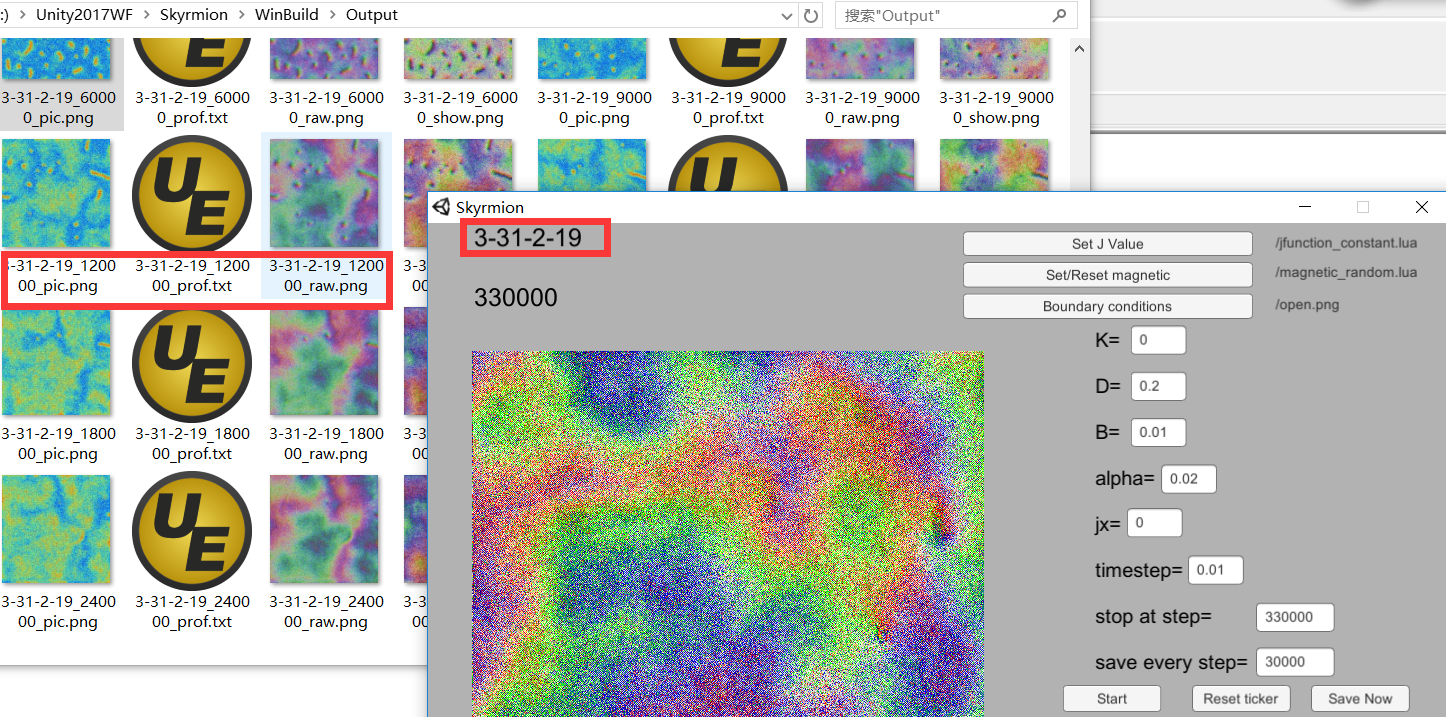
\includegraphics[scale=0.5]{intro4.png}
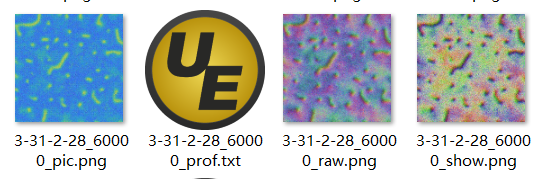
\includegraphics[scale=0.5]{output1.png}
\caption{\label{Fig:output}Output files.}
\end{figure}

The 'show.png` is the image shown in the program.

The 'raw.png` is a image with the RGB color set as $r=0.5\times n_x+0.5$, $g=0.5\times n_y+0.5$ and $b=0.5\times n_z+0.5$. Which can be used as input in for example matlab.

For example, the code
\lstset{language=Matlab,%
    %basicstyle=\color{red},
    breaklines=true,%
    morekeywords={matlab2tikz},
    keywordstyle=\color{blue},%
    morekeywords=[2]{1}, keywordstyle=[2]{\color{black}},
    identifierstyle=\color{black},%
    showstringspaces=false,%without this there will be a symbol in the places where there is a space
    numbers=left,%
    numberstyle={\tiny \color{black}},% size of the numbers
    numbersep=9pt, % this defines how far the numbers are from the text
    emph=[1]{for,end,break},emphstyle=[1]\color{red}, %some words to emphasise
    %emph=[2]{word1,word2}, emphstyle=[2]{style},
}
\begin{lstlisting}
imds = imageDatastore({'4-3-15-14_3300000_raw.png'});
img = readimage(imds,1);

nz=zeros(512,512);
for i=1:512
    for j=1:512
        nx=2.0*(double(img(i,j,1))/255.0) - 1.0;
        ny=2.0*(double(img(i,j,2))/255.0) - 1.0;
        nz(i,j)=2.0*(double(img(i,j,3))/255.0) - 1.0;
    end
end

x = 1:1:512;
y = 1:1:512;
[X,Y] = meshgrid(x,y);
Z = nz;
v = [cos(pi*exp(-1.0)),cos(pi*exp(-1.0))];

figure
imshow(img)
hold on;
contour(X,Y,Z,v,'linecolor','k')
\end{lstlisting}
will detect possible edge of a skyrmion, and the result is shown in Fig.~\ref{Fig:edge}.
\begin{figure}
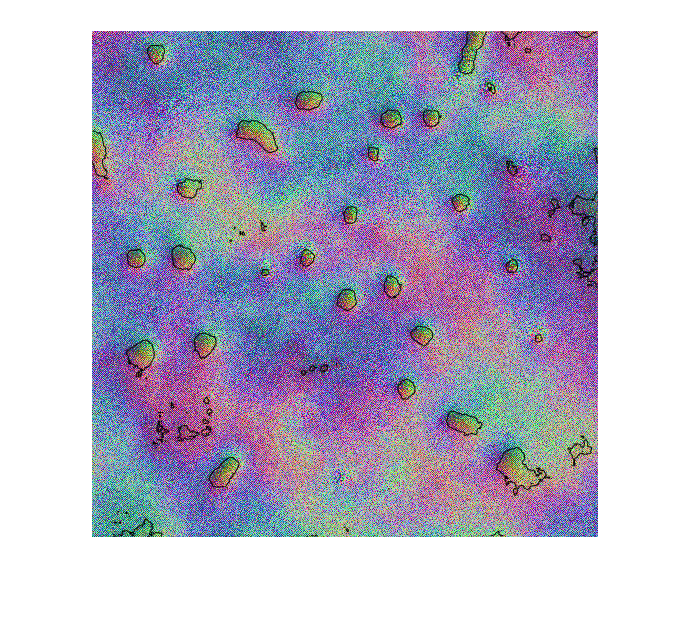
\includegraphics[scale=0.5]{edges.png}
\caption{\label{Fig:edge}Possible edge (NOTE: NOT Accurate!).}
\end{figure}

The content of the 'prof.txt` is the configuration of the simulation, for example
\begin{lstlisting}
start time=03-31-2018 02:28:46
step=120000
j value=/jfunction_constant.lua
initla magnetic=/magnetic_random.lua
boundary condition=/open.png
K=0
D=0.2
B=0.01
Gilbert alpha=0.02
Electric current jx=0
time step=0.01
\end{lstlisting}

The 'pic.png` is a illustration of the magnetic momentums. Part of it is shown in Fig.~\ref{Fig:output2}
\begin{figure}
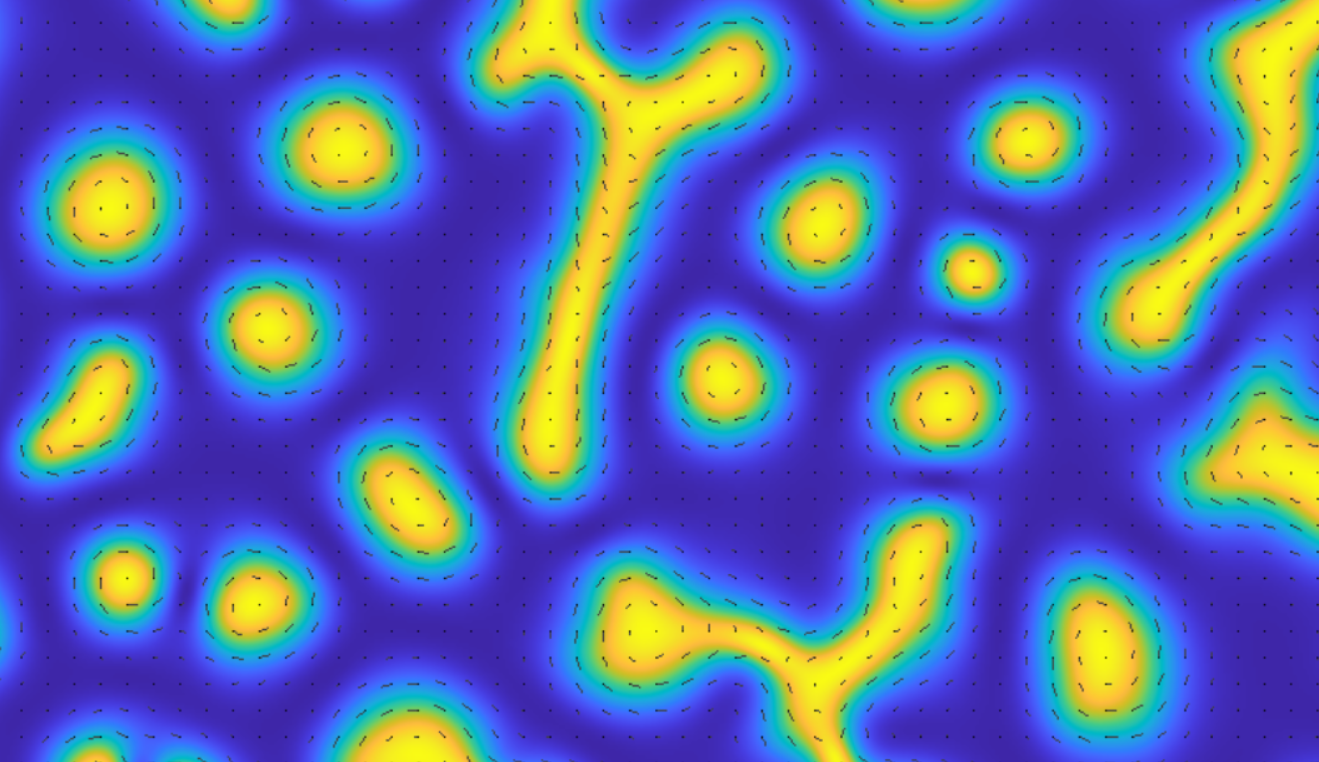
\includegraphics[scale=0.3]{output2.png}

\includegraphics[scale=0.5]{parula.png}
\caption{\label{Fig:output2}Illustration of the magnetic momentums. The color shows $n_z$. The color map is 'parula` in Matlab. The small black lines show $(n_x,n_y)$.}
\end{figure}

\section{\label{sec:6}An example of simulation}

\subsection{\label{sec:6.1}Start simulation}

Start from random, apply a large magnetic field to bake the momentums all up, like Fig.~\ref{Fig:start} and \ref{fig:result1}.
\begin{figure}
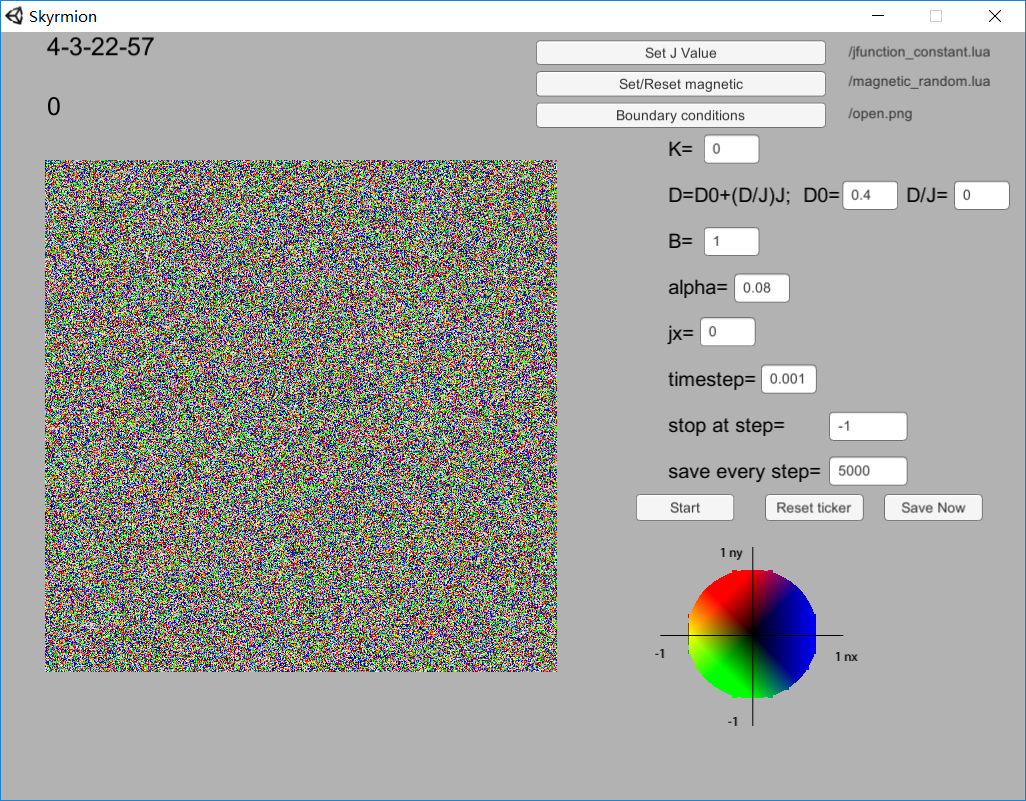
\includegraphics[scale=0.3]{start.png}
\caption{\label{Fig:start}Start simulation, $J=2.0$ is choosed.}
\end{figure}

\begin{figure}[htb]
\centering
\subfloat[$step=0$]{
\includegraphics[width=0.33\textwidth]{4-3-22-58_0_show.png}}\hfill
\subfloat[$step=5000$]{
\includegraphics[width=0.33\textwidth]{4-3-22-58_5000_show.png}}\hfill
\subfloat[$step=10000$]{
\includegraphics[width=0.33\textwidth]{4-3-22-58_10000_show.png}}\vfill
\subfloat[$step=15000$]{
\includegraphics[width=0.33\textwidth]{4-3-22-58_15000_show.png}}\hfill
\subfloat[$step=20000$]{
\includegraphics[width=0.33\textwidth]{4-3-22-58_20000_show.png}}\hfill
\subfloat[$step=25000$]{
\includegraphics[width=0.33\textwidth]{4-3-22-58_25000_show.png}}
\caption{All point up}
\label{fig:result1}
\end{figure}

\subsection{\label{sec:6.2}The stripes}

Then, remove the magnetic field, the results are shown in Fig.~\ref{fig:result2}

\begin{figure}[htb]
\centering
\subfloat[$step=0$]{
\includegraphics[width=0.24\textwidth]{4-3-22-59_0_show.png}}\hfill
\subfloat[$step=100000$]{
\includegraphics[width=0.24\textwidth]{4-3-22-59_100000_show.png}}\hfill
\subfloat[$step=200000$]{
\includegraphics[width=0.24\textwidth]{4-3-22-59_200000_show.png}}\hfill
\subfloat[$step=300000$]{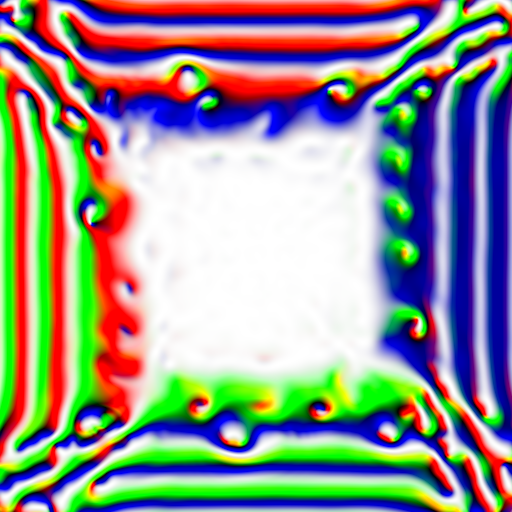
\includegraphics[width=0.24\textwidth]{4-3-22-59_300000_show.png}}\vfill
\subfloat[$step=400000$]{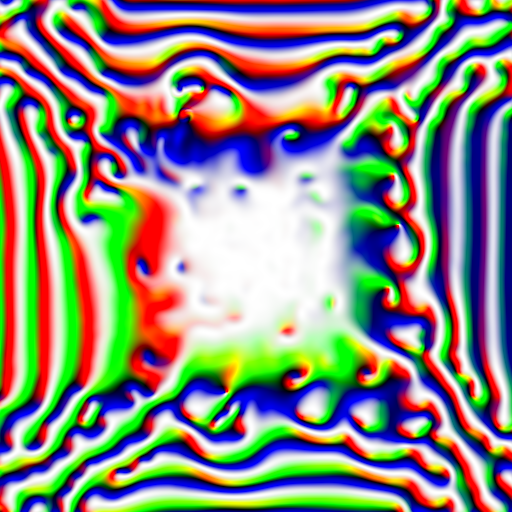
\includegraphics[width=0.24\textwidth]{4-3-22-59_400000_show.png}}\hfill
\subfloat[$step=500000$]{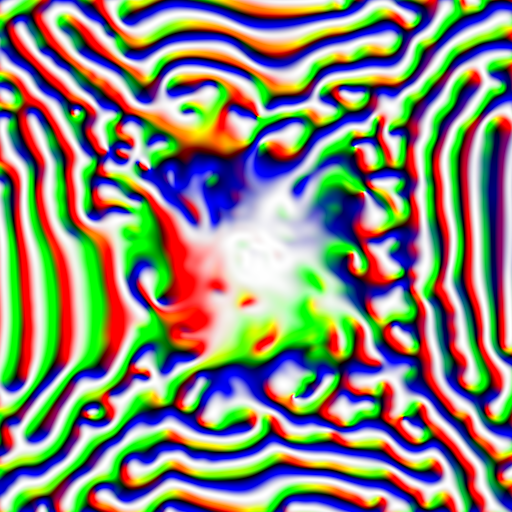
\includegraphics[width=0.24\textwidth]{4-3-22-59_500000_show.png}}\hfill
\subfloat[$step=600000$]{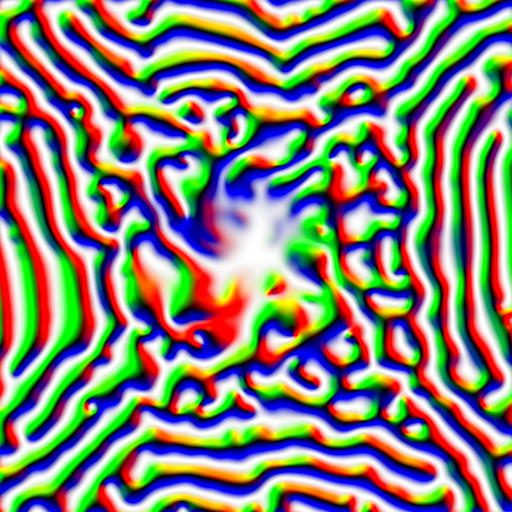
\includegraphics[width=0.24\textwidth]{4-3-22-59_600000_show.png}}\hfill
\subfloat[$step=700000$]{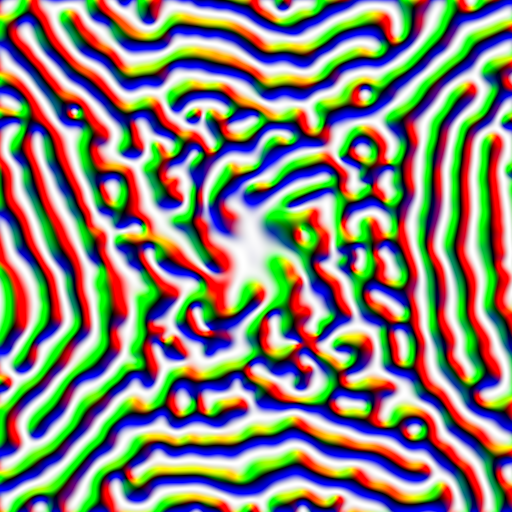
\includegraphics[width=0.24\textwidth]{4-3-22-59_700000_show.png}}\vfill
\subfloat[$step=800000$]{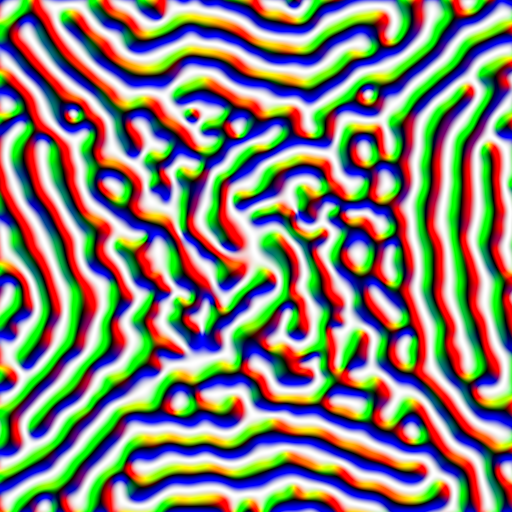
\includegraphics[width=0.24\textwidth]{4-3-22-59_800000_show.png}}\hfill
\subfloat[$step=900000$]{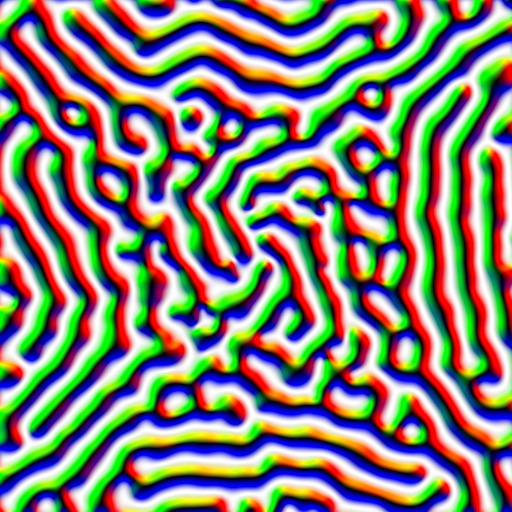
\includegraphics[width=0.24\textwidth]{4-3-22-59_900000_show.png}}\hfill
\subfloat[$step=1000000$]{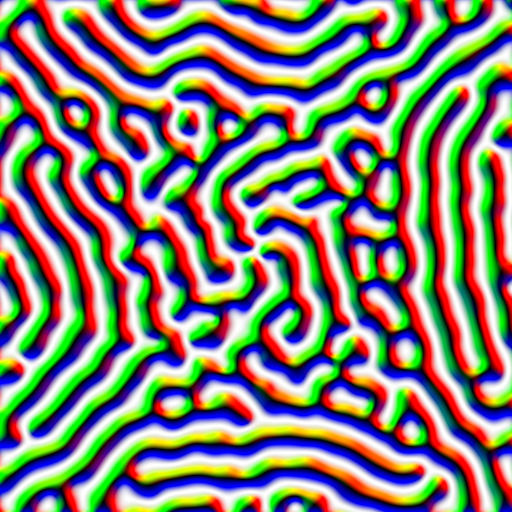
\includegraphics[width=0.24\textwidth]{4-3-22-59_1000000_show.png}}\hfill
\subfloat[$step=1100000$]{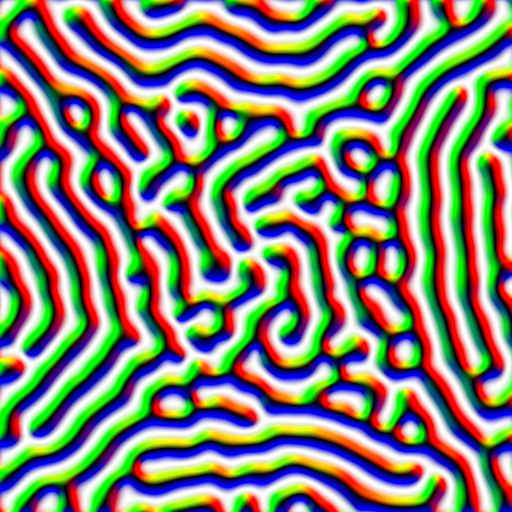
\includegraphics[width=0.24\textwidth]{4-3-22-59_1100000_show.png}}\vfill
\caption{Stripes}
\label{fig:result2}
\end{figure}

\subsection{\label{sec:6.3}The skyrmions}

Then, apply a small magnetic field, $B=0.1$ to see the stripes split into skyrmions as shown in Fig.~\ref{fig:result3}.

\begin{figure}[htb]
\centering
\subfloat[$step=0$]{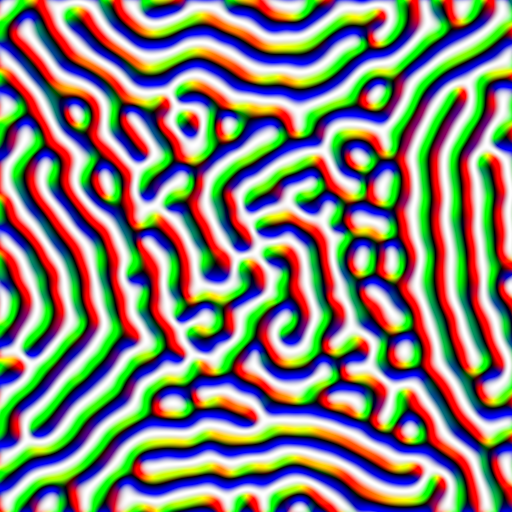
\includegraphics[width=0.24\textwidth]{4-3-23-26_0_show.png}}\hfill
\subfloat[$step=20000$]{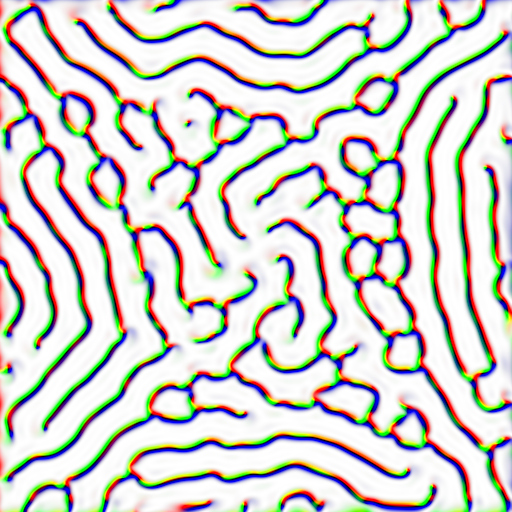
\includegraphics[width=0.24\textwidth]{4-3-23-26_20000_show.png}}\hfill
\subfloat[$step=40000$]{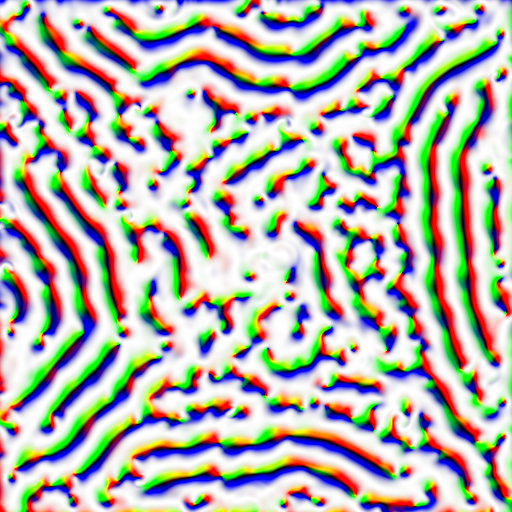
\includegraphics[width=0.24\textwidth]{4-3-23-26_40000_show.png}}\hfill
\subfloat[$step=60000$]{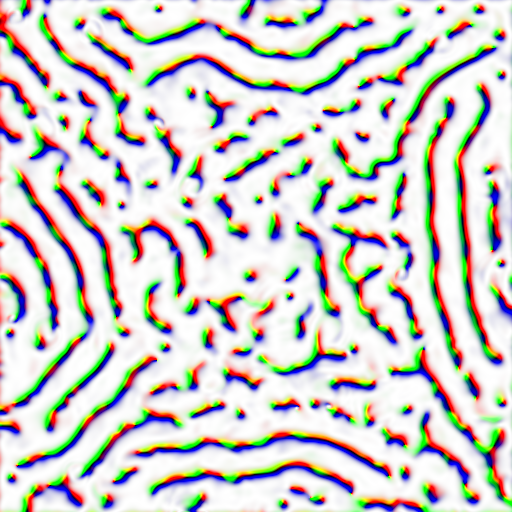
\includegraphics[width=0.24\textwidth]{4-3-23-26_60000_show.png}}\vfill
\subfloat[$step=80000$]{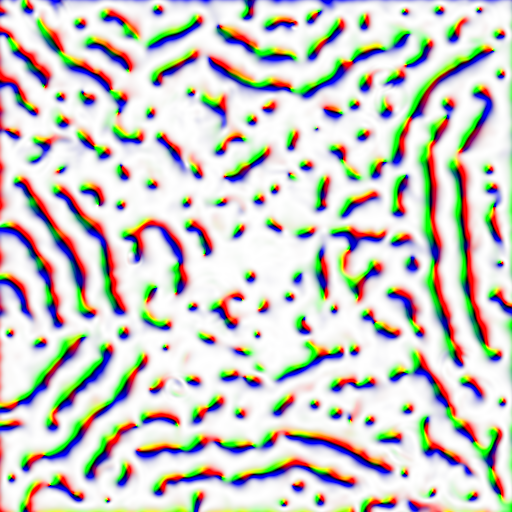
\includegraphics[width=0.24\textwidth]{4-3-23-26_80000_show.png}}\hfill
\subfloat[$step=100000$]{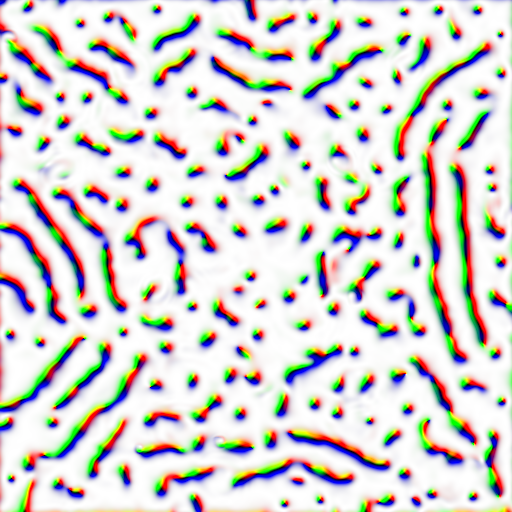
\includegraphics[width=0.24\textwidth]{4-3-23-26_100000_show.png}}\hfill
\subfloat[$step=120000$]{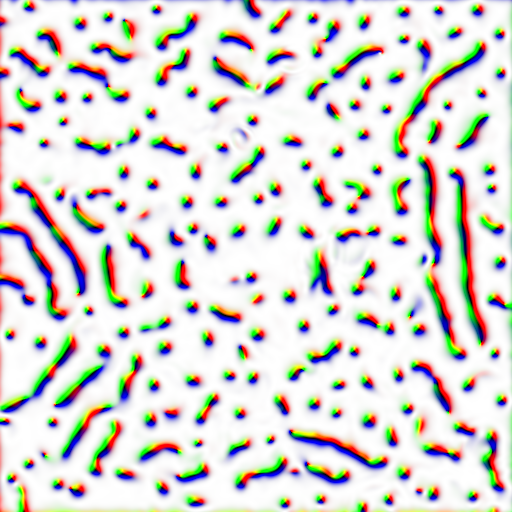
\includegraphics[width=0.24\textwidth]{4-3-23-26_120000_show.png}}\hfill
\subfloat[$step=140000$]{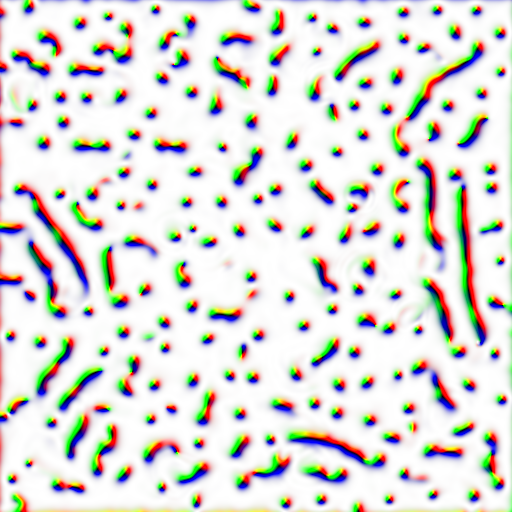
\includegraphics[width=0.24\textwidth]{4-3-23-26_140000_show.png}}\vfill
\subfloat[$step=160000$]{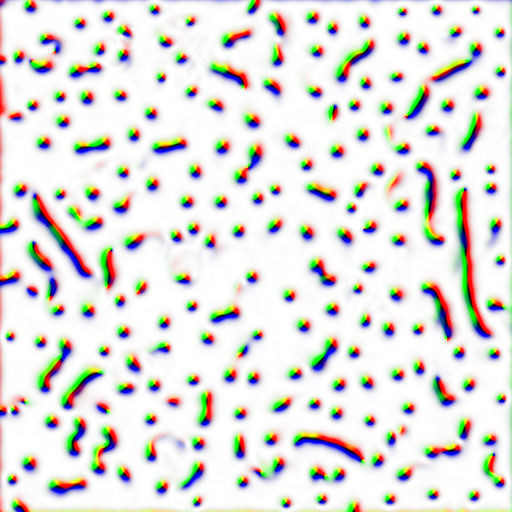
\includegraphics[width=0.24\textwidth]{4-3-23-26_160000_show.png}}\hfill
\subfloat[$step=180000$]{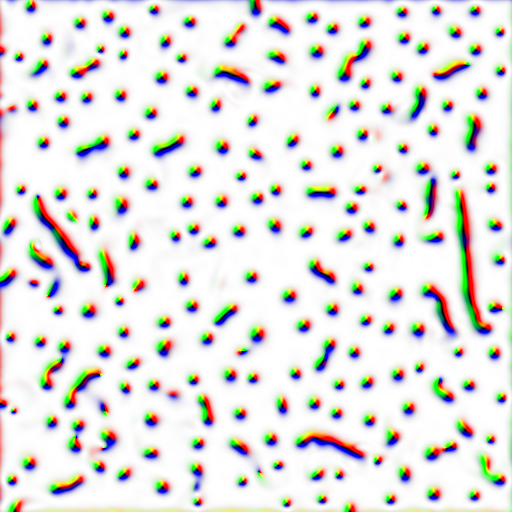
\includegraphics[width=0.24\textwidth]{4-3-23-26_180000_show.png}}\hfill
\subfloat[$step=200000$]{\includegraphics[width=0.24\textwidth]{4-3-23-26_200000_show.png}}\hfill
\subfloat[$step=220000$]{\includegraphics[width=0.24\textwidth]{4-3-23-26_220000_show.png}}\vfill
\caption{stripes split into skyrmions}
\label{fig:result3}
\end{figure}

\subsection{\label{sec:6.4}Moving skyrmions}

Then, apply a current, $j_x=1$ to see the motion of skyrmions, as shown in Fig.~\ref{fig:result4}.

\begin{figure}[htb]
\centering
\subfloat[$step=0$]{\includegraphics[width=0.24\textwidth]{4-3-23-29_0_show.png}}\hfill
\subfloat[$step=20000$]{\includegraphics[width=0.24\textwidth]{4-3-23-29_20000_show.png}}\hfill
\subfloat[$step=40000$]{\includegraphics[width=0.24\textwidth]{4-3-23-29_40000_show.png}}\hfill
\subfloat[$step=60000$]{\includegraphics[width=0.24\textwidth]{4-3-23-29_60000_show.png}}\vfill
\subfloat[$step=80000$]{\includegraphics[width=0.24\textwidth]{4-3-23-29_80000_show.png}}\hfill
\subfloat[$step=100000$]{\includegraphics[width=0.24\textwidth]{4-3-23-29_100000_show.png}}\hfill
\subfloat[$step=120000$]{\includegraphics[width=0.24\textwidth]{4-3-23-29_120000_show.png}}\hfill
\subfloat[$step=140000$]{\includegraphics[width=0.24\textwidth]{4-3-23-29_140000_show.png}}\vfill
\subfloat[$step=160000$]{\includegraphics[width=0.24\textwidth]{4-3-23-29_160000_show.png}}\hfill
\subfloat[$step=180000$]{\includegraphics[width=0.24\textwidth]{4-3-23-29_180000_show.png}}\hfill
\subfloat[$step=200000$]{\includegraphics[width=0.24\textwidth]{4-3-23-29_200000_show.png}}\hfill
\subfloat[$step=220000$]{\includegraphics[width=0.24\textwidth]{4-3-23-29_220000_show.png}}\vfill
\caption{Moving skyrmions}
\label{fig:result4}
\end{figure}


\end{document}
%
% ****** End of file template.aps ******
